%
% main.tex -- Paper zum Thema Polynome
%
% (c) 2019 Hochschule Rapperswil
%
\chapter{Wavelets und polynomiale Signale\label{chapter:polynomials}}
\lhead{Wavelets und polynomiale Signale}
\begin{refsection}
\chapterauthor{Raphael Nestler}

{\parindent=0pt
In} der Literatur zu Wavelets findet man die folgende Aussage zu Daubechies
Wavelets:
\index{Daubechies-Wavelet}%
\begin{displayquote}[\cite{wikipedia:daubechies}]
For example, $D2$, with one vanishing moment, easily encodes polynomials of one
coefficient, or constant signal components. $D4$ encodes polynomials with two
coefficients, i.e.\ constant and linear signal components; and $D6$ encodes
3-polynomials, i.e.\ constant, linear and quadratic signal components.
\end{displayquote}
Ein Daubechies Wavelet mit $A$ verschwindenden Momenten und Filterlänge $N=2A$
\index{Moment}%
sollte also ein Polynom der Ordnung $A-1$ einfach darstellen können. Wir wollen
\index{Ordnung}%
erörtern, was das nun in der Praxis genau bedeutet und welche Anwendungen es
ermöglicht.

\begin{figure}
    \centering
    % Filter mit 2 Ebenen

\usetikzlibrary{shapes,arrows}

\tikzset{%
  block/.style    = {draw, thick, rectangle, minimum height = 3em,
    minimum width = 3em},
  input/.style    = {coordinate}, % Input
  output/.style   = {coordinate} % Output
}
% Defining string as labels of certain blocks.
\newcommand{\suma}{\Large$+$}
\newcommand{\inte}{$\displaystyle \int$}
\newcommand{\derv}{\huge$\frac{d}{dt}$}

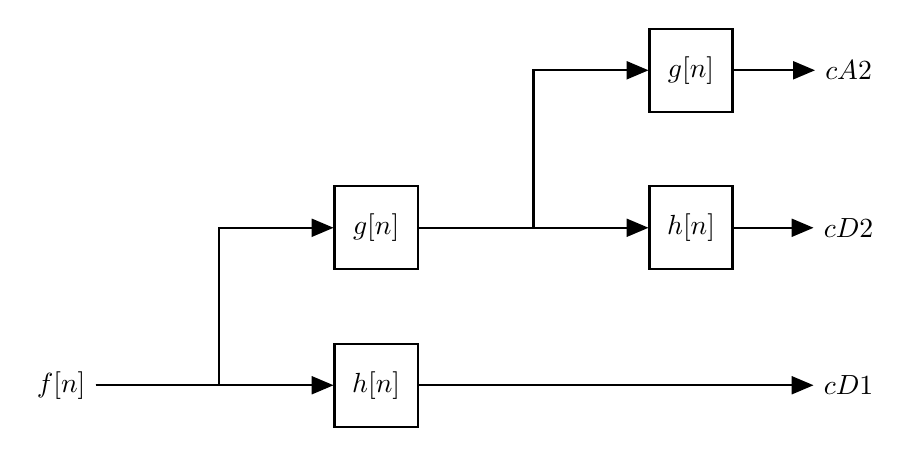
\begin{tikzpicture}[auto, thick, node distance=2cm, >=triangle 45]
\draw
	% Ebene 1
	node at (0,0)[name=in]{$f[n]$}
    node [input, right of=in](input1){}
	node [block, right of=input1] (h1) {$h[n]$}
	node [block, above of=h1] (g1) {$g[n]$}

	% Ebene 2
    node [input, right of=g1](input2){}
	node [block, right of=input2] (h2) {$h[n]$}
	node [block, above of=h2] (g2) {$g[n]$}

	% Ausgänge
    node [right of=g2](outg) {$cA2$}
    node [below of=outg](out2) {$cD2$}
    node [below of=out2](out1) {$cD1$}
;

    % Ebene 1
	\draw[->](in) -- node {}(h1);
	\draw[->](in) -- (input1) |- node {}(g1);
	\draw[->](h1) -- node {}(out1);

    % Ebene 2
	\draw[->](g1) -- node {}(h2);
	\draw[->](g1) -- (input2) |- node {}(g2);
	\draw[->](h2) -- node {}(out2);

	\draw[->](g2) -- node {}(outg);


\end{tikzpicture}
    \caption{Wavelet-Transformation als Filter.\label{polynomials:filter}}
\end{figure}

Im folgenden werden wir Daubechies Wavelets mit $A$ verschwindenden Momenten
mit db$A$ bezeichnen. Auch werden wir die Wavelet-Transformation als Filter
betrachten wie in \cref{haar:approximation:filter} beschrieben. Dabei werden
wir die Notation von Detail- und Approximationskoeffizienten verwenden. Die
Detailkoeffizienten auf Ebene $j$ ($cDj$) sind dabei der Ausgang des Hochpasses
\index{Detailkoeffizient}%
\index{Hochpass}%
$h$ und die Approximationskoeffizienten auf Ebene $j$ ($cAj$) der Ausgang des
\index{Approximationskoeffizient}%
\index{Tiefpass}%
Tiefpasses $g$.

Die Detailkoeffizienten auf Ebene $j$ entsprechen der Analyse mit einem $2^j$
skalierten Mutterwavelet $\psi$ und die Approximationskoeffizienten der
entsprechenden Analyse mit einem Vaterwavelet $\varphi$.

Die Analysen und Simulationen wurden jeweils mittels Python~\cite{python} und im
\index{Python}%
Speziellen dem PyWavelets~\cite{gregory_r_lee_2019_2634243} Paket durchgeführt.
\index{PyWavelets}%
Der dazu verwendete Code wurde in einem GitHub-Repository%
\footnote{\url{https://github.com/rnestler/mathsem-FS2019/tree/paper}}%
~\cite{polynomials:repo}
abgelegt. Zusätzlich sind auch interaktive Jupyter Notebooks vorhanden um den
\index{Jupyter}%
Einfluss von verschiedenen Parametern auszuprobieren. Mittels
Binder%
\footnote{\url{https://mybinder.org/v2/gh/rnestler/mathsem-FS2019/paper}}%
~\cite{project_jupyter-proc-scipy-2018}
\index{Binder}%
kann eine Online-Umgebung gestartet werden um diese Beispiele auszuführen.

\section{Analyse von polynomialen Signalen}
\rhead{Polynomiale Signale}

Als erstes werden wir die Signale in \cref{polynomials:signals} mittels des db1
(Haar) Wavelets analysieren.
\begin{figure}
    \centering
    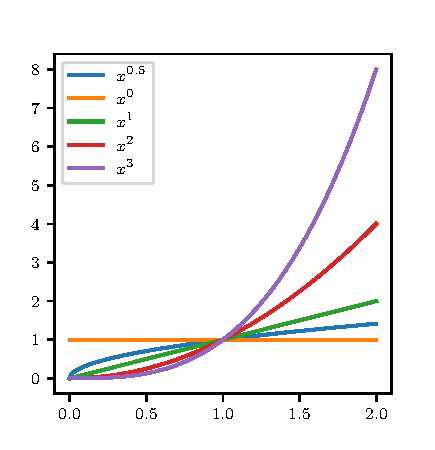
\includegraphics{papers/polynomials/images/polynomials_signals.pdf}
    \caption{Die verschiedenen zu analysierenden polynomialen Signale.\label{polynomials:signals}}
\end{figure}
In~\cref{polynomials:haar} sind die Approximations- und die Detailkoeffizienten
der Transformation zu sehen. Wir sehen, dass die Approximationskoeffizienten
uns das grobe Signal und im Fall von $x^0 = 1$ sogar das exakte Signal liefern.
Die Detailkoeffizienten scheinen uns etwas zu liefern was proportional zur
ersten Ableitung des Signals ist. In \cref{polynomials:diff} sind zum Vergleich
die Ableitungen der verschiedenen Signale gegeben.

\begin{figure}
    \centering
    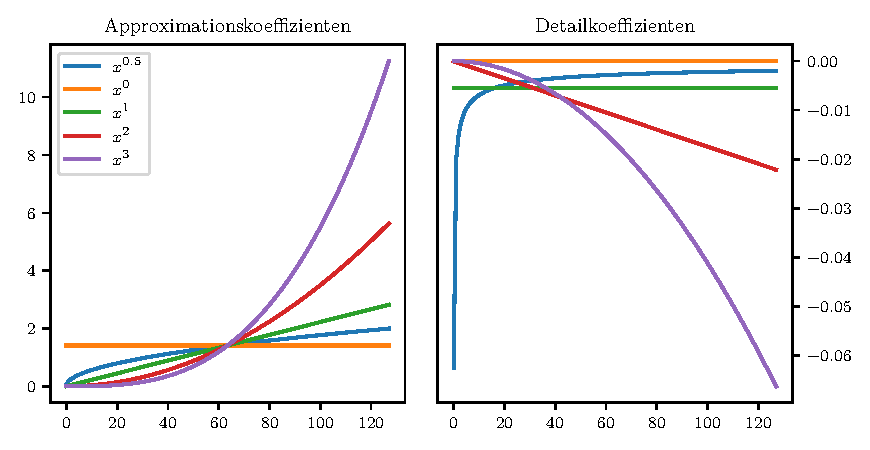
\includegraphics{papers/polynomials/images/polynomials_signals_db1.pdf}
    \caption{Analyse der Polynome mit db1 (Haar) Wavelet. Die
             Detailkoeffizienten sind proportional zur
             Ableitung.\label{polynomials:haar}}
\end{figure}

\begin{figure}
    \centering
    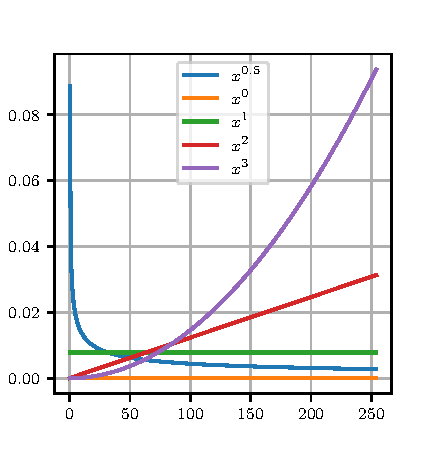
\includegraphics{papers/polynomials/images/polynomials_signals_diff.pdf}
    \caption{Ableitungen der Polynome.\label{polynomials:diff}}
\end{figure}

Dieses Verhalten ist zu erwarten wenn man bedenkt, dass das Haar Wavelet
\index{Haar-Wavelet}%
jeweils die Summe und die Differenz zweier benachbarter Samples analysiert.
Siehe dazu auch \cref{haar:allwavelets:image} im Kapitel zum Haar Wavelet. Aus
\cref{fast:akoefgleichung} von \cref{section:fast} wissen wir, dass die
Approximationskoeffizienten $cA_{j,k}$ und die Detailkoeffizienten $dA_{j,k}$
folgendermassen gebildet werden:
\begin{align}
cA_{j+1,k}
&=
\frac{1}{\sqrt{2}} \sum_{l\in\mathbb Z} \bar{h}_l cA_{j,k+l}, \nonumber
\\
cD_{j+1,k}
&=
\frac{1}{\sqrt{2}} \sum_{l\in\mathbb Z} \bar{g}_l cA_{j,k+l}.
\label{polynomials:cD_haar}
\end{align}
Setzen wir nun in \cref{polynomials:cD_haar} die $g$ Koeffizienten $g_0=1$ und
$g_1=-1$ des Haarwavelet und die Samples $f(x_k)$ und $f(x_{k + 1})$ ein,
erhalten wir die Detailkoeffizienten
\begin{align}
    cD_{1,k} & = \frac{1}{\sqrt{2}}\left(f(x_k) - f(x_{k + 1})\right).
\end{align}
Vergleichen wir diese mit dem Differenzenquotienten
\begin{align}
\frac{\Delta y}{\Delta x} &= \frac{f(x_0+\Delta x) - f(x_0)}{\Delta x}
                           = \frac{f(x_{k+1}) - f(x_k)}{x_{k+1} - x_k} \nonumber \\
                          &= cD_{1,k} \frac{-\sqrt{2}}{x_{k+1} - x_k},
                          \label{polynomials:eq:cD_haar_ableitung}
\end{align}
als Approximation der Ableitung,
\index{Ableitung}%
stellt sich heraus, dass sie dem mit $-\frac{\sqrt{2}}{\Delta x}$ skalierten
Detailkoeffizienten entspricht.

Nun stellt sich die Frage: Was passiert wenn wir Daubechies Wavelets mit mehr
verschwindenden Momenten zur Analyse einsetzen? In \cref{polynomials:db2_3}
sind jeweils die Detailkoeffizienten der Analyse mit db2 und db3 Wavelet zu
sehen.
\begin{figure}
    \centering
    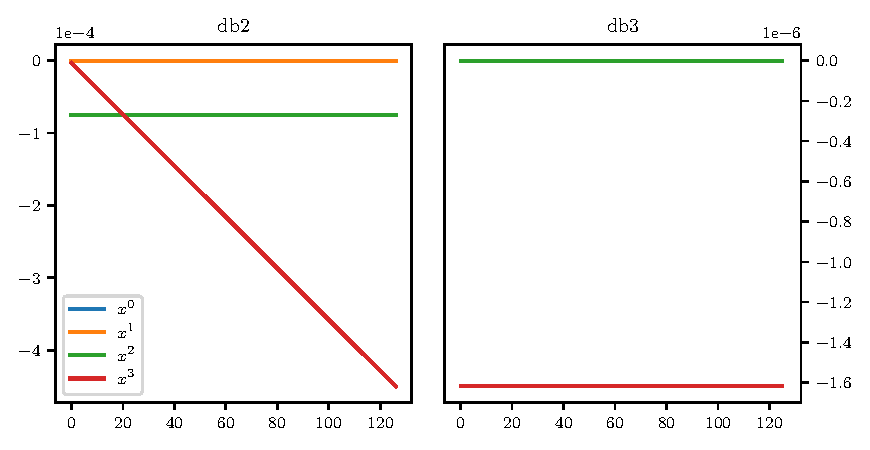
\includegraphics{papers/polynomials/images/polynomials_signals_db2_3.pdf}
    \caption{Detailkoeffizienten der Analyse mit db2/3 Wavelet. Sie sind
             proportional zur zweiten und dritten Ableitung der
             Polynome.\label{polynomials:db2_3}}
\end{figure}
Wie sich herausstellt, liefern diese Wavelets jeweils Detailkoeffizienten,
welche proportional zur zweiten und dritten Ableitung der Polynome ist.

Warum ist das so? Betrachten wir zuerst einmal algebraisch, wie sich konstante
und lineare Funktionen mit den Daubechies Wavelets verhalten.

\subsection{Konstante Funktionen}
Die Detailkoeffizienten konstanter Funktionen $f(x) = a$ ergeben sich direkt
aus \cref{polynomials:cD_haar}:
\begin{align*}
    cD &= \frac{1}{\sqrt{2}} \sum_{l\in\mathbb Z} \bar{g}_l a \\
       &= \frac{a}{\sqrt{2}} \sum_{l\in\mathbb Z} \bar{g}_l.
\end{align*}
Da die Summe der $\bar{g}_l$ immer 0 ist, werden die Detailkoeffizienten für
konstante Funktionen also immer 0 sein für alle beliebigen Wavelets.

\subsection{Lineare Funktionen}

Für lineare Funktionen der Form $f(x) = a + b x$ ergeben sich bei Analyse mit
dem Haar Wavelet die Detailkoeffizienten
\begin{align*}
    cD = \frac{1}{\sqrt{2}} [ (a + b x) - (a + b (x + \Delta x)) ]
    = \frac{- b \Delta x}{\sqrt{2}}.
\end{align*}
Diese entsprechen, wie bereits in \cref{polynomials:eq:cD_haar_ableitung}
gezeigt, der skalierten Ableitung der Funktion.

Bei der Analyse mit dem db2 Wavelet ergeben sich die Detailkoeffizienten
\begin{align*}
    cD &= \sum_{l=0}^{3} g_l (a + b (x + l\Delta x)) \\
       &= g_0 (a + b x) + g_1 (a + b (x + \Delta x)) + g_2 (a + b (x + 2 \Delta x)) + g_3 (a + b (x + 3 \Delta x)) \\
       &= (g_0 + g_1 + g_2 + g_3) (a + bx) + b \Delta x (g_1 + 2 g_2 + 3 g_3).
\end{align*}
Da $(g_0 + g_1 + g_2 + g_3) = 0$ bleibt noch $(g_1 + 2 g_2 + 3 g_3)$. Wenn wir
nun die Koeffizienten des db2 Wavelet aus \cref{section:daubechies} einsetzen,
erhalten wir
\begin{align*}
    g_1 + 2 g_2 + 3 g_3 &= \frac{3 + \sqrt{3}}{4\sqrt{2}} + 2 \frac{-3 + \sqrt{3}}{4\sqrt{2}} + 3 \frac{1 - \sqrt{3}}{4\sqrt{2}} = 0.
\end{align*}
Die Detailkoeffizienten verschwinden somit komplett bei der Analyse von
linearen Funktionen mit dem db2 Wavelet.

Für quadratische Funktionen der Form $a + bx + cx^2$ ergeben sich bei der
Analyse mit dem db2 Wavelet analog die Detailkoeffizienten \[cD =
-\sqrt{\frac{3}{2}} c \Delta x^2.\] Diese sind somit proportional zur zweiten
Ableitung $\frac{2c x}{\Delta x^2}$ der Funktion.

Wir könnten dies weiterführen für Polynome und Daubechies Wavelets höherer
Ordnung $A$. Es würde ersichtlich, dass immer die Terme niedriger Ordnung
verschwinden und von den Termen der Ordnung $A$ etwas proportionales zur
$A$-ten Ableitung entsteht. Dieses Verhalten ist ein Resultat davon wie die
Daubechies Wavelets erzeugt werden. Sehen wir uns dazu
\cref{definition:ordnung}
\begin{align*}
    \int_{\mathbb R} t^k\psi(t)\,dt=0\quad \text{für $k<N$}
\end{align*}
aus \cref{section:ordnung} an. Diese gilt als Bedingung für die Daubechies
Wavelets und zeigt, dass alle Terme $t^k$ niedriger Ordnung bei der Analyse mit
dem Mutterwavelet $\psi$ verschwinden.

\subsection{Beliebige analytische Funktionen}

In diesem Abschnitt wollen wir zeigen, dass die Daubechies Wavelets eine
Approximation der Ableitung beliebiger analytischer Funktionen liefern können.
Eine analytische Funktion lässt sich nämlich als Taylorreihe darstellen:
\index{Taylor-Reihe}%
\begin{align*}
    f(x) = T f(x; a) & = \sum_{n=0}^\infty  \frac{f^{(n)}(a)}{n!} (x-a)^n = f(a) + f'(a) (x-a) + \frac{f''(a)}{2}(x-a)^2 + \frac{f'''(a)}{6} (x-a)^3 + \cdots.
\end{align*}
Der Einfachheit halber werden wir im folgenden die Entwicklungsstelle $a=0$
verwenden. Für die Taylorreihe ergibt sich somit
\begin{align*}
    f(x) = T f(x; 0) & = \sum_{n=0}^\infty  \frac{f^{(n)}(0)}{n!} x^n = f(0) + f'(0) x + \frac{f''(0)}{2}x^2 + \frac{f'''(0)}{6} x^3 + \cdots.
\end{align*}

Analysieren wir nun ein solches Polynom mit einem db$A$ ($\mathcal{W}_{dbA}$)
so werden die Terme der Ordnung $A-1$ verschwinden. Es können also nur noch der
Term der Ordnung $A$ welcher die A-te Ableitung liefert und die Terme
höherer Ordnung einen Einfluss auf die Detailkoeffizienten haben:
\begin{align*}
    cD &= \mathcal{W}_{dbA} \sum_{n=A}^\infty \frac{f^{(n)}(0)}{n!} x^n \\
       &= \mathcal{W}_{dbA} \frac{f^{A}(0)}{A!}x^A + \mathcal{W}_{dbA}\sum_{n=A+1}^\infty \frac{f^{(n)}(0)}{n!} x^n.
\end{align*}
Wenn der Restterm \[R_A = \sum_{n=A+1}^\infty \frac{f^{(n)}(0)}{n!} x^n\] nun
\index{Restterm}%
vernachlässigbar klein ist, liefern uns die Detailkoeffizienten eine
zuverlässige Approximation für die Ableitung beliebiger analytischer
Funktionen.

Wir wollen das am Beispiel der Exponentialfunktion $\exp(x)$ erläutern. Die
\index{Exponentialfunktion}
Taylorreihe der Exponentialfunktion ist
\begin{align*}
    e^{x} = \sum^{\infty}_{n=0} \frac{x^n}{n!} = 1 + x + \frac{x^2}{2!} + \frac{x^3}{3!} + \cdots.
\end{align*}
An der Stelle $x=0.1=10^{-1}$ ausgewertet ergibt sich
\begin{align*}
    e^{0.1} = \sum^{\infty}_{n=0} \frac{0.1^n}{n!} = 1 + 10^{-1} + \frac{10^{-2}}{2!} + \frac{10^{-3}}{3!} + \cdots.
\end{align*}
Wollen wir nun die dritte Ableitung mit dem db3 Wavelet berechnen, ist der Term
$\frac{10^{-3}}{3!}$ relevant. Der nächste Term $\frac{10^{-4}}{4!}$ ist schon
um Faktor 40 kleiner. Je nach Anwendung haben diese Terme somit weniger
Einfluss auf das Resultat als etwaiges Rauschen. Ist nur eine qualitative
Aussage zur Ableitung des Signals gefordert, kann die Approximation ebenfalls
bereits den Anforderungen genügen.

Daubechies Wavelets mit $A$ verschwindenden Momenten können uns also direkt die
$A$-te Ableitung von Polynomen der Ordnung $A$ liefern. Für beliebige
analytische Funktionen können sie uns eine gute Approximation zur Ableitung
liefern, sofern die Taylorreihe genügend schnell konvergiert und der Restterm
entsprechend klein ist.

\section{Anwendung zur rauscharmen Ableitung}
\rhead{Rauscharme Ableitung}
\index{Ableitung!rauscharm}%

Beim diskreten Ableiten (Differenzieren) von Signalen stellt sich oftmals das
Problem, dass Rauschen im Signal verstärkt wird. Anstelle der Ableitung des
interessanten Signals sehen wir also nur die zufällige Ableitung des Rauschens.
Dies wird zudem verstärkt, wenn ein Signal mehrfach abgeleitet werden soll.
\cref{polynomials:noise:signals} zeigt unsere ursprünglichen polynomialen
Signale mit leichtem Rauschen versehen und die Ableitung davon. Wie erwartet
ist die Ableitung vom Rauschen dominiert und die Steigung des ursprünglichen
Polynoms ist kaum noch erkennbar.

\begin{figure}
    \centering
    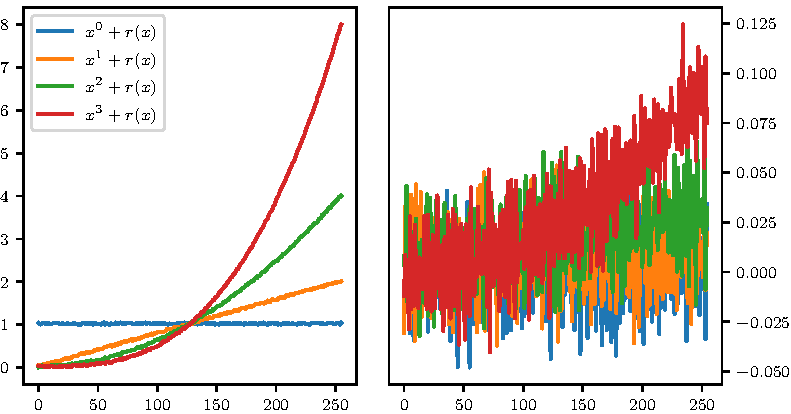
\includegraphics{papers/polynomials/images/polynomials_noise_signals.pdf}
    \caption{Verrauschte Signale und deren Ableitung. Die Ableitung ist
             dominiert vom Rauschen und die Steigung der Polynome ist kaum noch
             zu erkennen.\label{polynomials:noise:signals}}
\end{figure}

\subsection{Erste Ableitung mit Haar Wavelet}

Was passiert nun wenn die verrauschten Signale mit einem Haar Wavelet
analysieren werden? Wie in \cref{polynomials:noise:db1} zu sehen bringt dies
noch keine wesentliche Verbesserung zum direkten Ableiten. Die
Detailkoeffizienten sind vom Rauschen dominiert und der Anteil welcher
proportional zur Ableitung ist, ist kaum mehr erkennbar.

\begin{figure}
    \centering
    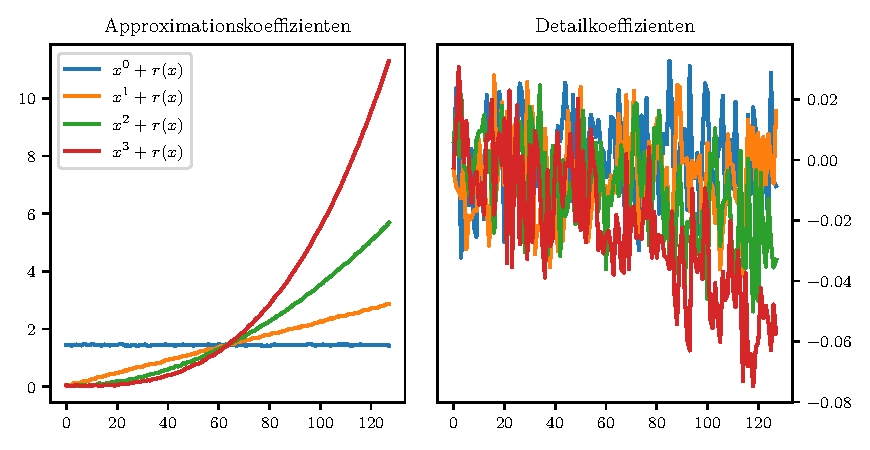
\includegraphics{papers/polynomials/images/polynomials_noise_db1.pdf}
    \caption{Analyse verrauschter Signale mit Haar Wavelet. Die
             Detailkoeffizienten sind dominiert vom Rauschen. Der Anteil
             welcher proportional zur Ableitung der Polynome ist, ist kaum
             erkennbar.\label{polynomials:noise:db1}}
\end{figure}

Nun können wir aber mit dem Wavelet eine Multiskalenanalyse durchführen. Im
Fall vom Haar Wavelet ist dies vergleichbar damit, dass zuerst der Mittelwert
gebildet und dann abgeleitet wird. Aus \cref{fast:akoefgleichung} von
\cref{section:fast} wissen wir, dass die Approximationskoeffizienten $cA_{j,k}$
und die Detailkoeffizienten $dA_{j,k}$ folgendermassen gebildet werden:
\begin{align}
cA_{j+1,k}
&=
\frac{1}{\sqrt{2}} \sum_{l\in\mathbb Z} \bar{h}_l cA_{j,k+l},
\nonumber \\
cD_{j+1,k}
&=
\frac{1}{\sqrt{2}} \sum_{l\in\mathbb Z} \bar{g}_l cA_{j,k+l}.
\end{align}
Im Fall vom Haar-Wavelet entspricht das
\begin{align}
cA_{j+1,k}
&=
\frac{1}{\sqrt{2}} (cA_{j,k} + cA_{j,k+1}),
\nonumber \\
cD_{j+1,k}
&=
\frac{1}{\sqrt{2}} (cA_{j,k} - cA_{j,k+1}).
\end{align}

Nehmen wir nun das Signal mit den Abtastwerten $\{a_{0,0}, a_{0,1}, a_{0,2},
a_{0,3}\}$ so ergeben sich für die erste Ebene die Approximationskoeffizienten
\begin{align}
cA_{1,0}
&=
\frac{1}{\sqrt{2}} (a_{0,0} + a_{0,1})\qquad\text{und}
\nonumber \\
cA_{1,1}
&=
\frac{1}{\sqrt{2}} (a_{0,2} + a_{0,3}).
\end{align}
Die zweite Ebene wird dann aus den Approximationskoeffizienten der ersten Ebene
berechnet. Für die Approximations- und Detailkoeffizienten erhalten wir dann
\begin{align}
cA_{2,0}
&=
\frac{1}{\sqrt{2}} (cA_{1,0} + cA_{1,1})
=
\frac{1}{2} (a_{0,0} + a_{0,1}) + \frac{1}{2} (a_{0,2} + a_{0,3})\qquad \text{und}
\nonumber \\
cD_{2,0}
&=
\frac{1}{\sqrt{2}} (cA_{1,0} - cA_{1,1})
=
\frac{1}{2} (a_{0,0} + a_{0,1}) - \frac{1}{2} (a_{0,2} + a_{0,3}).
\end{align}
Die Detailkoeffizienten entsprechen somit der Differenz der Mittelwerte zweier
benachbarter Abtastwerte.

\begin{figure}
\centering
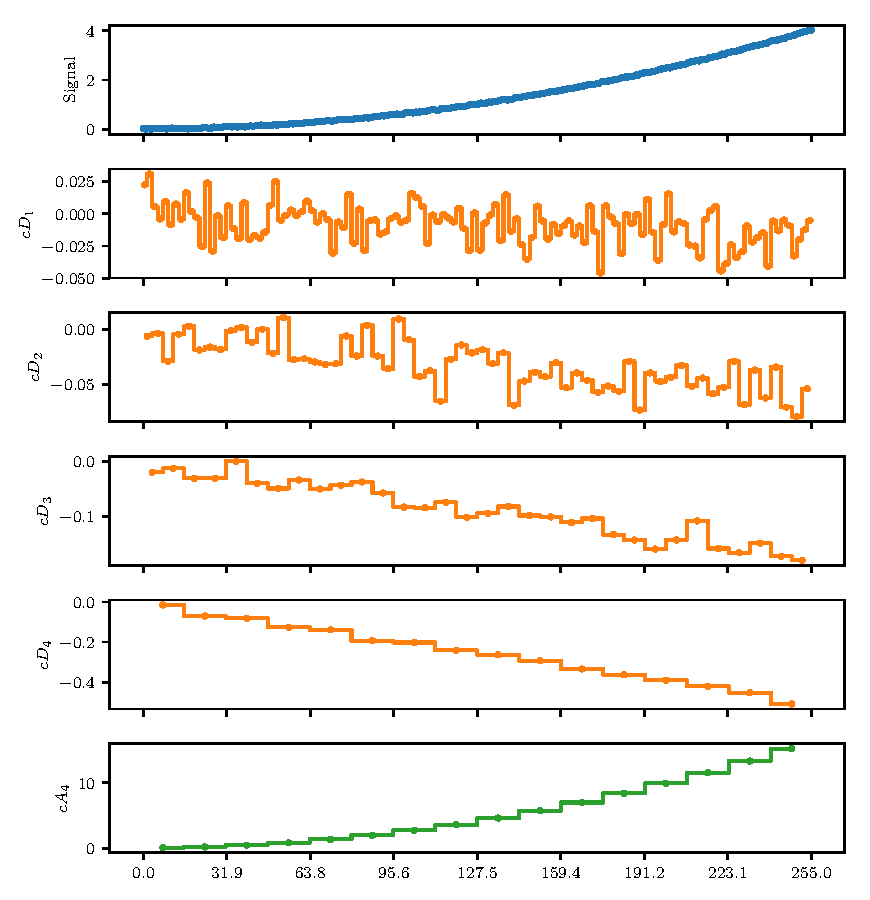
\includegraphics{papers/polynomials/images/polynomials_noise_db1_multi.pdf}
\caption{Multiskalenanalyse von $x^2 + r(x)$ mit Haar Wavelet.\\
Blau: Signal mit den einzelnen Samples\\
Orange: Detailkoeffizienten $cD_{1-4}$ \\
Grün: Approximationskoeffizienten $cA_4$\\
Die Detailkoeffizienten der Stufe 4 sind kaum noch vom Rauschen
betroffen und approximieren die Ableitung des Ursprungssignals gut.
Jedoch ist die zeitliche Auflösung reduziert.\label{polynomials:noise:db1_multi}}
\end{figure}
\begin{figure}
\centering
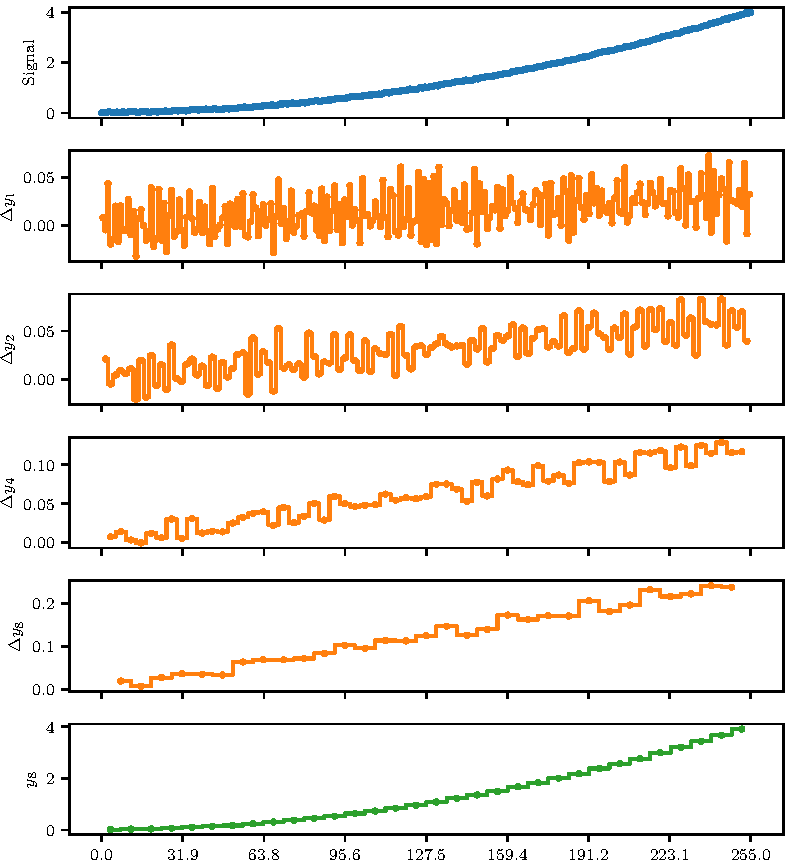
\includegraphics{papers/polynomials/images/polynomials_noise_moving_average.pdf}
\caption{Ableitung nach Mittelwertbildung.\\
Blau: Signal mit den einzelnen Samples\\
Orange: Ableitungen nach Mittelwertbildung über 1, 2, 4 und 8 Samples\\
Grün: Mittelwerte über 8 Samples\\
Die zeitliche Auflösung ist doppelt so hoch im Vergleich zu der
Multiskalenanalyse mit dem Haar Wavelet.\label{polynomials:noise:average}}
\end{figure}
\begin{figure}
\centering
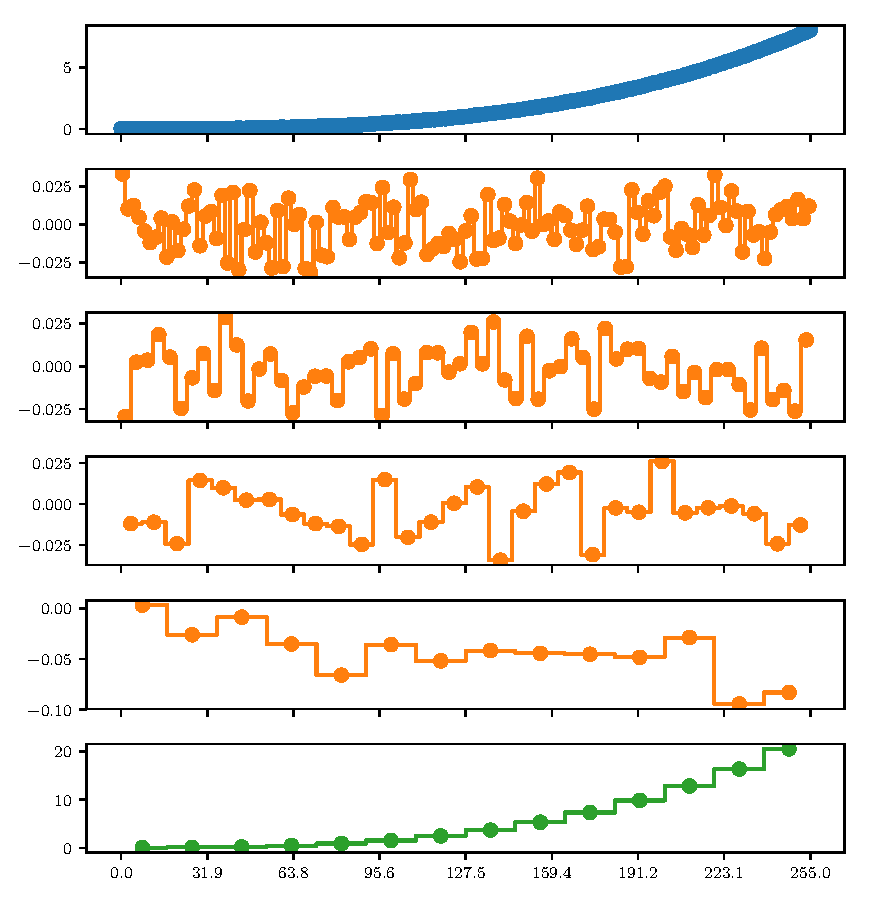
\includegraphics{papers/polynomials/images/polynomials_noise_db2_multi.pdf}
\caption{Multiskalenanalyse von $x^3 + r(x)$ mit db2 Wavelet. \\
Blau: Signal mit den einzelnen Samples\\
Orange: Detailkoeffizienten $cD_{1-4}$ \\
Grün: Approximationskoeffizienten $cA_4$\label{polynomials:noise:db2_multi}}
\end{figure}
\begin{figure}
\centering
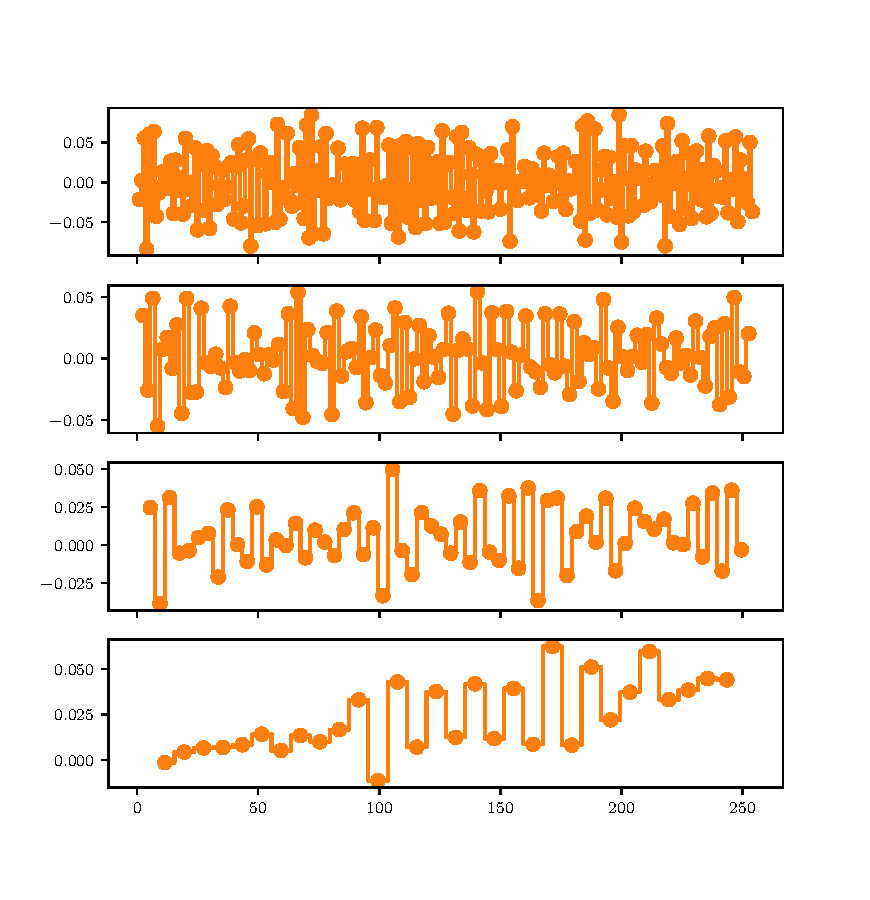
\includegraphics{papers/polynomials/images/polynomials_noise_moving_average_2nd.pdf}
\caption{Zweite Ableitung nach Mittelwertbildung.\\
Blau: Signal mit den einzelnen Samples\\
Orange: Ableitungen nach Mittelwertbildung über 1, 2, 4 und 8 Samples\\
Grün: Mittelwerte über 8 Samples\label{polynomials:noise:average2nd}}
\end{figure}
In \cref{polynomials:noise:db1_multi} ist das Signal $x^2 + r(x)$, die
Detailkoeffizienten der verschiedenen Stufen der Multiskalenanalyse mit dem
Haar Wavelet und dann noch die Approximationskoeffizienten der letzten Stufe
abgebildet. Es ist zu sehen, dass die Detailkoeffizienten mit höherer Stufe
eher der Ableitung des originalen Polynoms entsprechen und weniger vom Rauschen
betroffen sind. Jedoch nimmt die zeitliche Auflösung ab.
Die Stufenbreite macht jeweils den zeitlichen Bereich, also die Anzahl Samples,
welcher für die Berechnung des jeweiligen Koeffizienten relevant ist sichtbar.

Im Vergleich dazu sind in \cref{polynomials:noise:average} die direkte
Ableitung und die Ableitungen nach der Mittelwertbildung über 2, 4 und 8 Werte
zu sehen. Auffällig ist die höhere zeitliche Auflösung, da im Gegensatz zur
Methode mit den Wavelets kein Downsampling durchgeführt wird. Ansonsten zeigen
die beiden Verfahren wie erwartet das gleiche Verhalten bezüglich
Rauschresistenz.

\subsection{Zweite Ableitung mit db2 Wavelet}

Nun haben wir aber durch das Verfahren mit den Wavelets den Vorteil, dass wir
bei entsprechender Wahl des Wavelets mit $A$ verschwindenden Momenten direkt
die $A$-te Ableitung berechnen können.
In \cref{polynomials:noise:db2_multi} ist das Signal $x^3 + r(x)$, die
Detailkoeffizienten der verschiedenen Stufen der Multiskalenanalyse mit dem db2
Wavelet und die Approximationskoeffizienten der letzten Stufe abgebildet.
Es zeigt sich ein ähnliches Verhalten wie schon bei der Berechnung der ersten
Ableitung.

Im Vergleich dazu sind in \cref{polynomials:noise:average} die direkt
berechnete zweite Ableitung und die zweite Ableitungen nach der
Mittelwertbildung über 2, 4 und 8 Werte zu sehen.
Wieder liefern uns beide Verfahren ähnliche Resultate. Da die Daubechies
Wavelets höherer Ordnung im Vergleich zum einfachen Mitteln des
Ursprungssignals ein anderes Verhalten aufweisen, ist ein direkter Vergleich
nicht mehr so einfach möglich. Je nach Anwendung könnte aber das
Frequenzverhalten der Daubechies Wavelets einen Vorteil bieten.

Daubechies Wavelets bieten also eine komfortable Methode um verrauschte Signale
abzuleiten. Die Multiskalenanalyse kann dabei einen Kompromiss zwischen
Empfindlichkeit gegenüber Rauschen und zeitlicher Auflösung bieten.

Die Anwendung zur Ableitung kann auf der Binder Plattform im
\texttt{Ableitungen.ipynb} Notebook%
\footnote{\url{https://mybinder.org/v2/gh/rnestler/mathsem-FS2019/paper?filepath=Ableitungen.ipynb}}
nachvollzogen werden.

\section{Hochfrequente Anteile in Polynomen}
\rhead{Hochfrequente Anteile in Polynomen}

Im vorherigen Abschnitt lag der Fokus vor allem auf der Analyse des Polynoms
und dessen Ableitung. Die hochfrequenten Teile, also das Rauschen, wollten wir
dabei möglichst loswerden. Was nun aber wenn wir ein hochfrequentes Signal aus
einem sonst polynomialen Signal extrahieren wollen? Solche Signale könnten zum
Beispiel so wie in \cref{polynomials:sin:signals} aussehen. Da die Daubechies
Wavelets polynomiale Signale schon komplett in den Approximationskoeffizienten
darstellen können, sollten wir das interessante Signal direkt in den
Detailkoeffizienten sehen können.

\begin{figure}
    \centering
    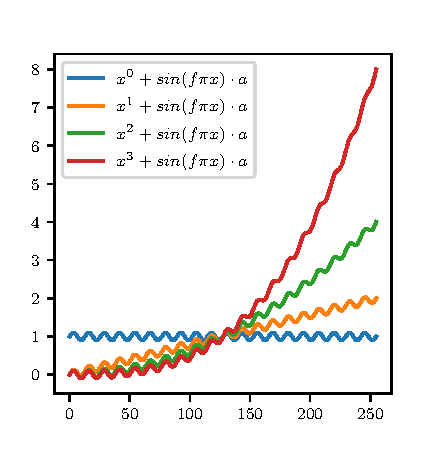
\includegraphics{papers/polynomials/images/polynomials_sin_signals.pdf}
    \caption{Polynomiale Signale mit überlagertem Sinus.\label{polynomials:sin:signals}}
\end{figure}

In \cref{polynomials:sin:db2} ist die Analyse mit dem db2 Wavelet zu sehen. Die
Detailkoeffizienten werden von dem enthaltenen Sinussignal dominiert. Das
Sinussignal lässt sich so also bestens extrahieren.

\begin{figure}
    \centering
    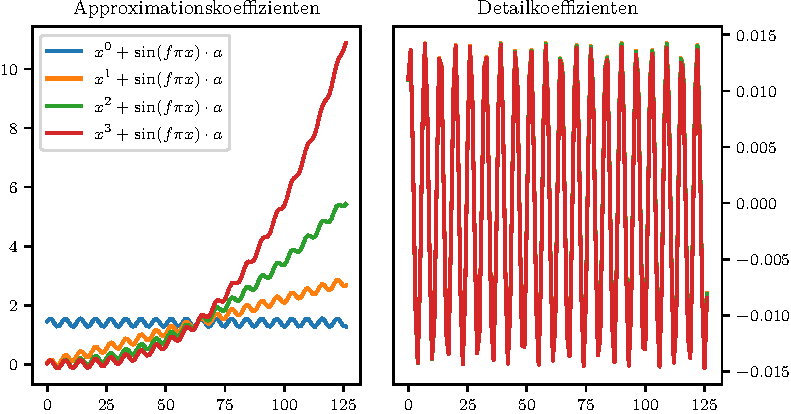
\includegraphics{papers/polynomials/images/polynomials_sin_db2.pdf}
    \caption{Analyse mit db2 Wavelet. Die Detailkoeffizienten sind dominiert
             vom Sinus Signal welches sich somit zuverlässig extrahieren
             lässt.\label{polynomials:sin:db2}}
\end{figure}

Wenn man an sinusförmigen Signalen interessiert ist, liegt es auch nahe die
diskrete Fourier-Transformation zu verwenden. In \cref{polynomials:sin:fft}
sind die Resultate der DFT zu sehen.
\begin{figure}
    \centering
    %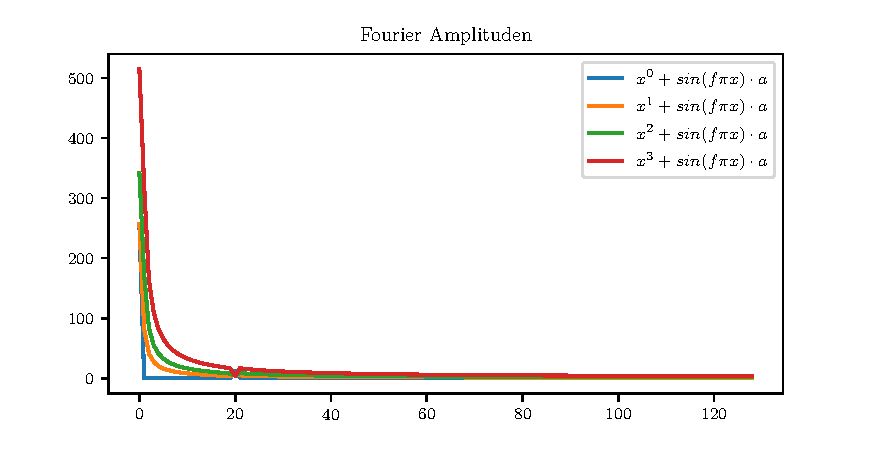
\includegraphics{papers/polynomials/images/polynomials_sin_fft.pdf}
    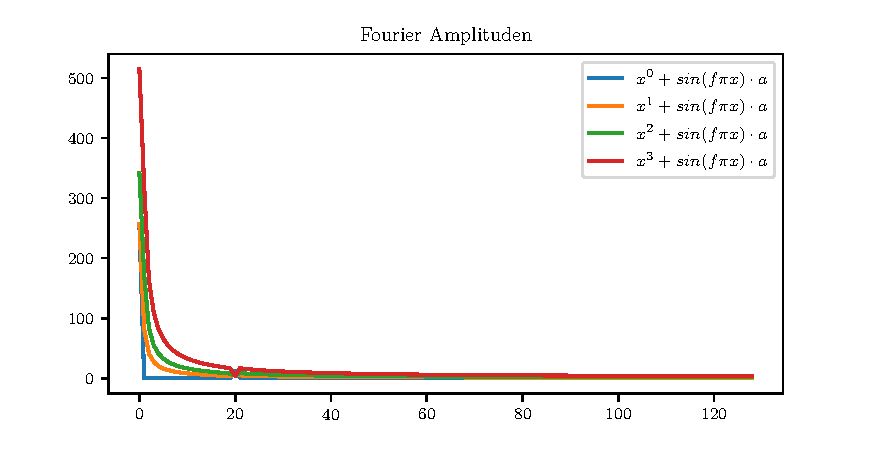
\includegraphics[width=\hsize]{papers/polynomials/images/polynomials_sin_fft.pdf}
    \caption{Analyse mit Fourier-Transformation. Die Frequenzanteile des
             Polynoms dominieren die Resultate. Der Peak bei $f=20$ kann leicht
             übersehen werden.\label{polynomials:sin:fft}}
\end{figure}
Dabei wird sichtbar, dass die Fourier-Koeffizienten des Polynoms dominieren und
dass der Peak bei 20, welcher durch den Sinus entsteht, unter geht. Dies ist
verständlich, wenn man bedenkt wie die Fourierreihen von Polynomen aussehen.
Nehmen wir als Beispiel das Polynom $f(x) = x$. Im Bereich $[0, 1]$ entspricht
es einer Sägezahnfunktion. Die Fourierreihe eines Sägezahns ist \[f(x) =
\index{Sägezahn}%
\frac{1}{2} - \frac{1}{\pi} \sum{\frac{1}{n} \sin(2 n \pi x)}.\] Nun ist
ersichtlich, dass die Fourier-Transformierte jede Frequenz $n$ mit
$\frac{1}{n}$ skaliert enthalten wird.

Die Analyse mittels Fourier-Transformation kann natürlich durch die Wahl einer
passenden Fensterfunktion (z.B. Hamming) zu besseren Resultaten führen. Dies
hat jedoch den Nachteil das zeitlich kurz auftretende Signale, je nach
Fenstergrösse und Position, unterschiedlich gedämpft werden.

Ein weiterer Vorteil der Wavelet-Transformation ist, dass sie uns auch den
Zeitpunkt liefert, bei dem das Signal aufgetreten ist.
\cref{polynomials:sin:padded} zeigt die Resultate einer Wavelet-Analyse mit
einem zeitlich lokalisierten Sinussignal.
\begin{figure}
    \centering
    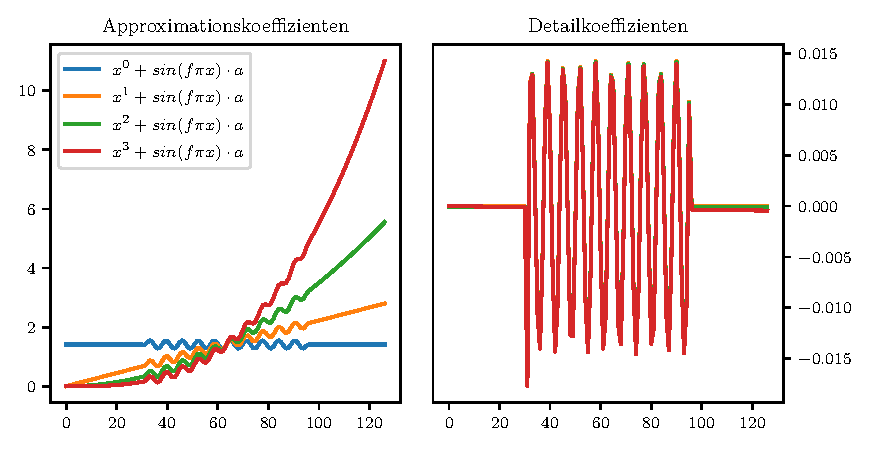
\includegraphics{papers/polynomials/images/polynomials_sin_padded_db2.pdf}
    \caption{Analyse mit db2 Wavelet eines zeitlich lokalisierten
             Sinussignals. Die Detailkoeffizienten sind dominiert vom
             überlagerten Sinussignal, welches sich so zuverlässig extrahieren
             lässt.\label{polynomials:sin:padded}}
\end{figure}
Die Anteile der Polynome ist in den Detailkoeffizienten im Vergleich zum
Sinussignal vernachlässigbar klein. Dies gilt auch bei der Analyse mit
Daubechies Wavelets mit wenig verschwindenden Momenten von Polynomen höherer
Ordnung. Zu sehen ist lediglich ein ganz schwacher Anstieg der
Detailkoeffizienten am Ende des Signals.

Die Analyse dieser Signale mit Daubechies Wavelets und DFT kann im
\texttt{Analyse von Sinus Signalen.ipynb} Notebook%
\footnote{\url{https://mybinder.org/v2/gh/rnestler/mathsem-FS2019/paper?filepath=Analyse\%20von\%20Sinus\%20Signalen.ipynb}}
nachvollzogen werden.

\section{Schlussfolgerung}
\rhead{Schlussfolgerung}
Ziel dieser Arbeit war, einen Überblick über die Eigenschaften der Daubechies
Wavelets zu bekommen. Wir konnten zeigen, dass Daubechies Wavelets mit $A$
verschwindenden Momenten Polynome der Ordnung $A-1$ schon komplett durch ihre
Skalierungfunktion $\varphi$ darstellen können. Als Folge daraus zeigte sich,
dass Polynome der Ordnung $A$ abgeleitet werden können.

In der Anwendung zum rauscharmen Ableiten konnten wir zeigen, dass Daubechies
Wavelets einen guten Kompromiss zwischen Rauschempfindlichkeit und zeitlicher
Auflösung der Ableitung liefern können. Interessant wäre zu untersuchen,
welche Effekte die Filtereigenschaften der Daubechies Wavelets höherer Ordnung
im Vergleich zum einfachen Mitteln und mehrfachen Ableiten von verrauschten
Signalen hat.

Es zeigte sich auch, dass Daubechies Wavelets sich hervorragend eignen um
hochfrequenten Anteilen aus polynomialen Signalen zu extrahieren. Das könnte
zum Beispiel interessant sein um Events in einem Prozess zu detektieren bei
welchem bekannt ist dass er sich linear oder exponentiell verhalten sollte.

\printbibliography[heading=subbibliography]
\end{refsection}
